\chapter{Introduction}\label{ch:introduction}

Ce manuel d'exploitation couvre les blocs instruments numériques \ReplicaGenOne{} et \ReplicaNextLong{} destinés aux Volkswagen Golf~II, Jetta~II et Scirocco~II.
Il résume les variantes matérielles, décrit leurs fonctions et explique comment installer, configurer, utiliser, stocker et entretenir les tableaux de bord.
Les recommandations s'adressent aux propriétaires de véhicules, aux électriciens automobiles et aux ateliers qui rétrofitent le produit.

Les chapitres suivants présentent le schéma d'identification du produit, les brochages des connecteurs, les conditions de fonctionnement ainsi que des procédures détaillées d'installation et de configuration.
Des sections de maintenance et de dépannage pour les deux générations de Replica sont également incluses afin que le bloc compteur puisse être entretenu sans la documentation d'usine.

\begin{figure}[htbp]
    \centering
    \begin{subfigure}{0.48\textwidth}
        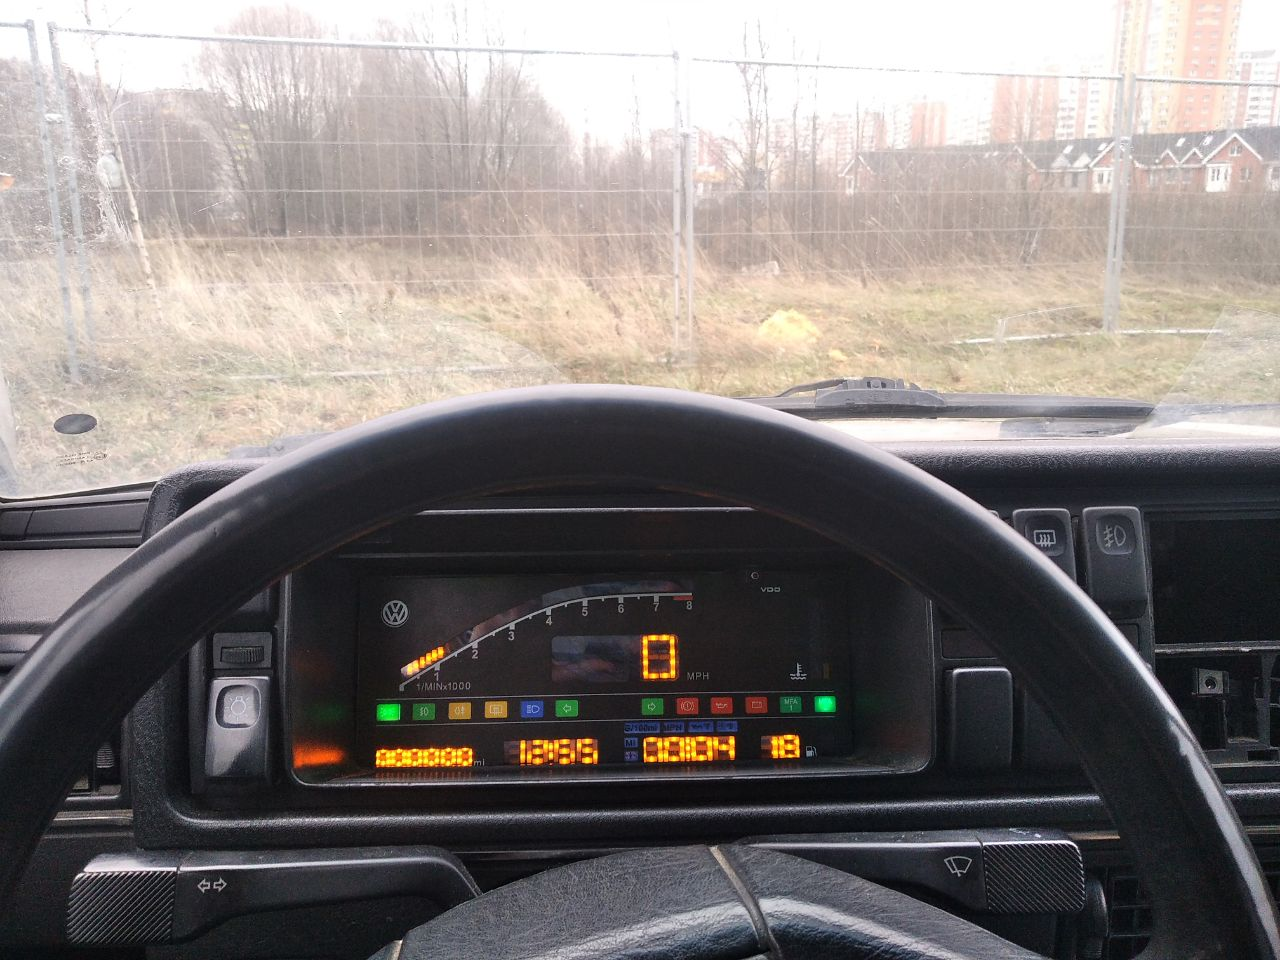
\includegraphics[width=\linewidth]{digifiz_manual/image004.jpg}
        \caption{Ensemble de livraison pour la configuration GART~8--MGF.}
    \end{subfigure}\hfill
    \begin{subfigure}{0.48\textwidth}
        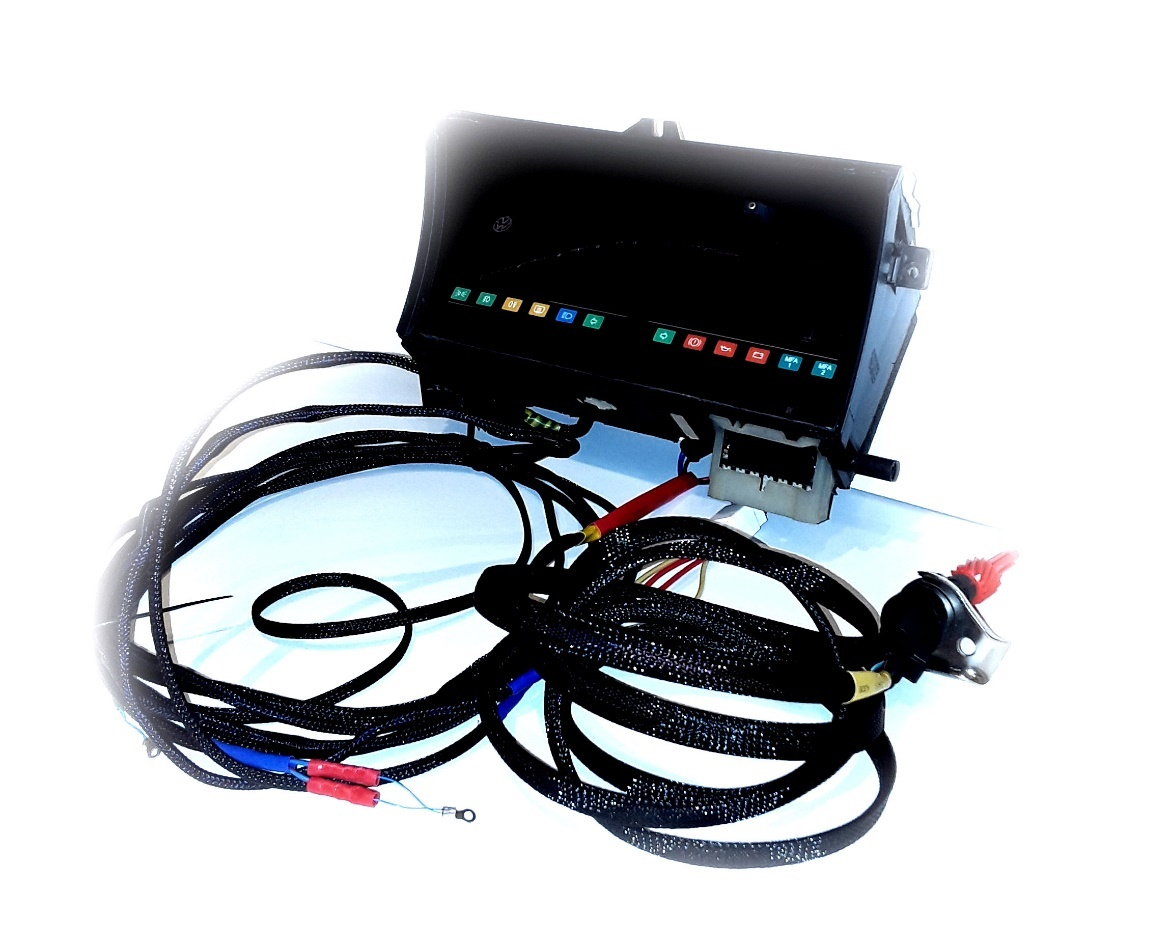
\includegraphics[width=\linewidth]{digifiz_manual/image005.jpg}
        \caption{Contenu typique d'un colis GART.}
    \end{subfigure}
    \begin{subfigure}{0.48\textwidth}
        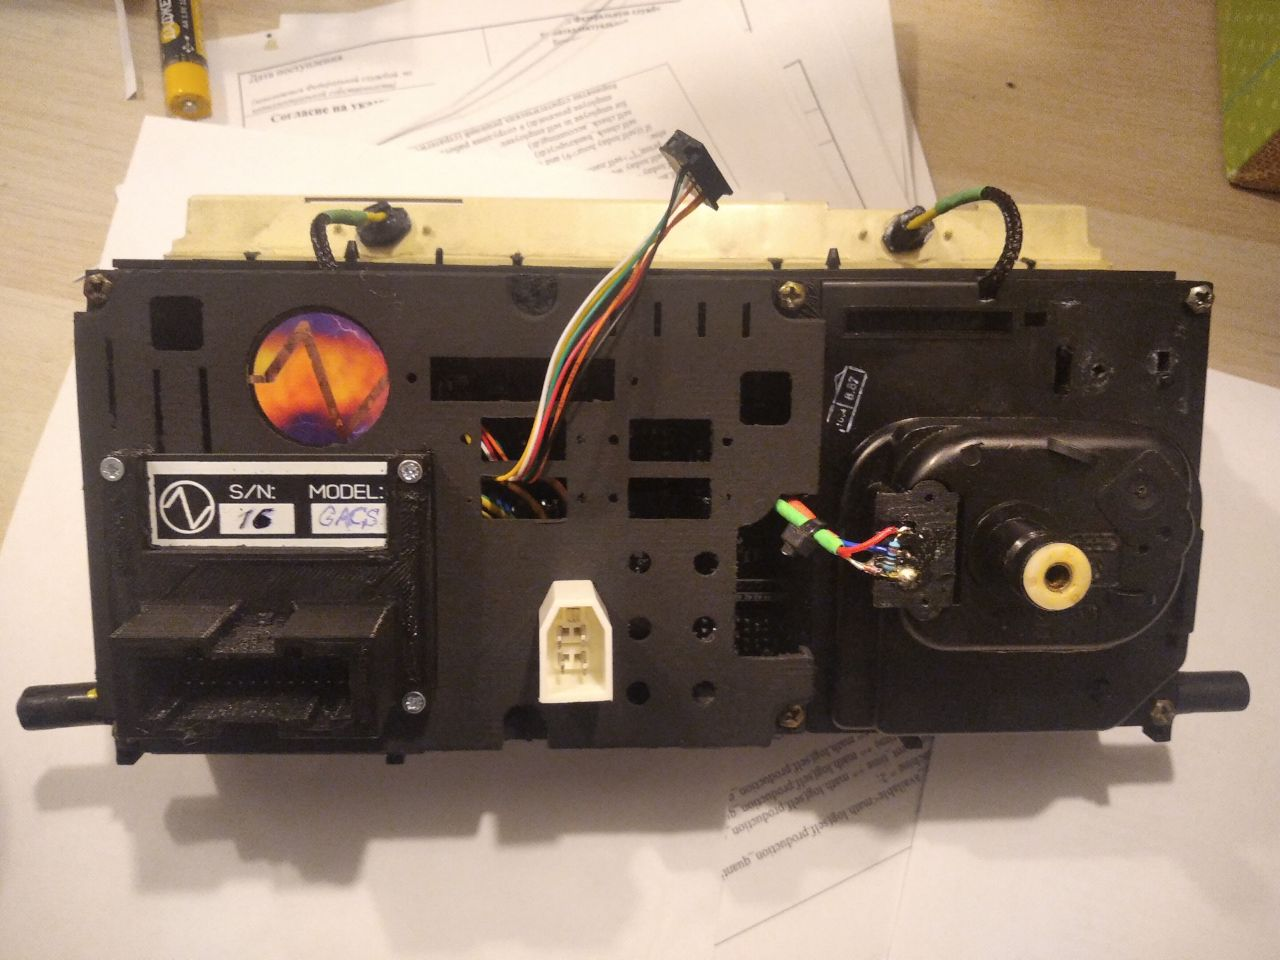
\includegraphics[width=\linewidth]{digifiz_manual/image006.jpg}
        \caption{Vue arrière de l'ensemble GACS à connecteur unique.}
    \end{subfigure}\hfill
    \begin{subfigure}{0.48\textwidth}
        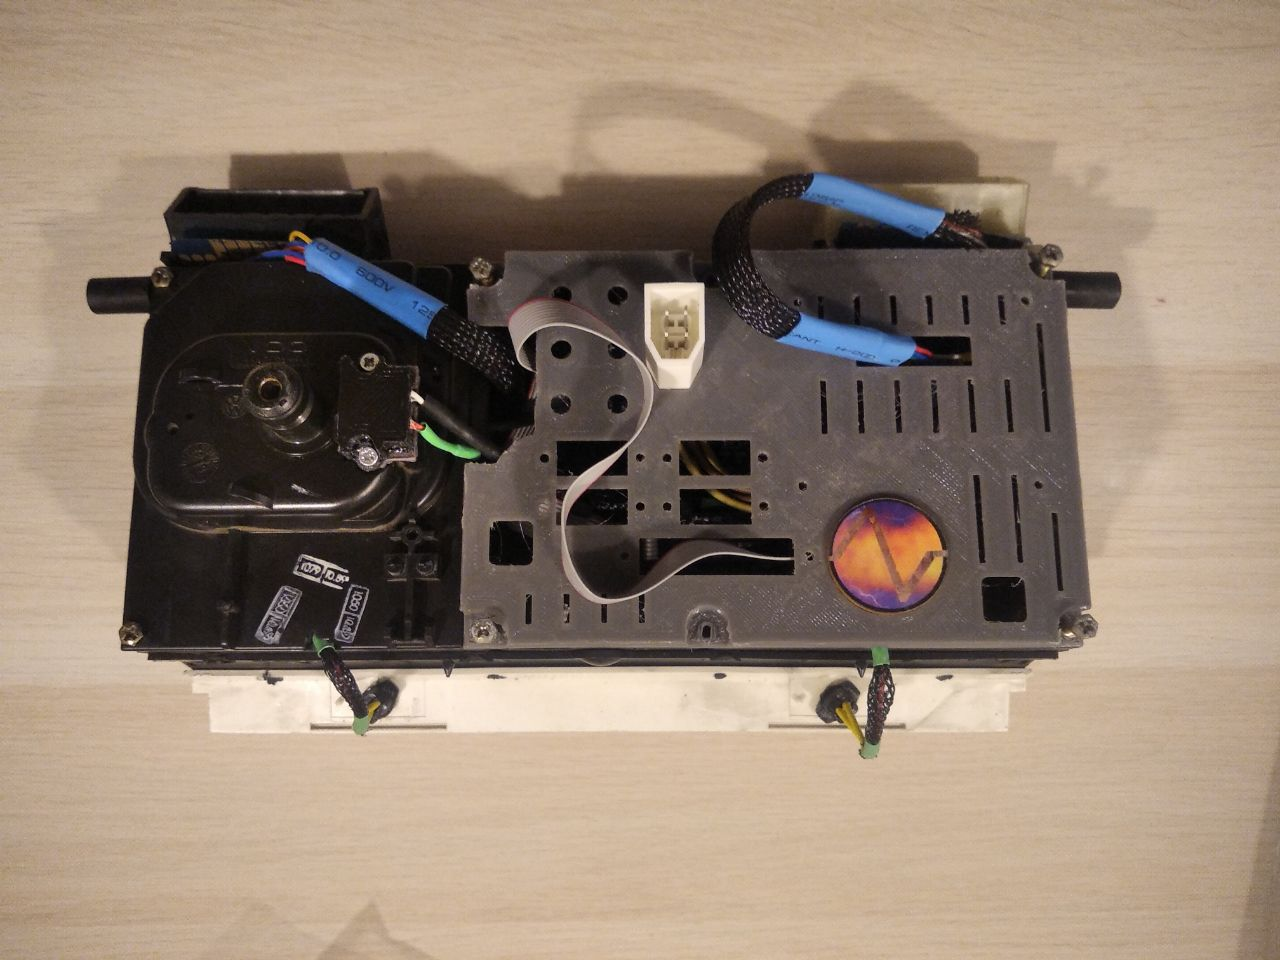
\includegraphics[width=\linewidth]{digifiz_manual/image007.jpg}
        \caption{Vue arrière de l'ensemble GACT à double connecteur.}
    \end{subfigure}
    \caption{Tableaux de bord \ReplicaGenOne{} et \ReplicaNextLong{} représentatifs fournis avec ce manuel.}
\end{figure}

Chaque variante est livrée avec les composants nécessaires à la chaîne cinématique visée, aux unités de mesure et au style de faisceau.
Les chapitres suivants déchiffrent les marquages des variantes et fournissent les tableaux de connecteurs afin que le bloc puisse être intégré en toute sécurité.
